\documentclass[12pt]{article}
\usepackage{amsmath, amssymb, circuitikz, graphicx}
\usepackage[margin=1in]{geometry}
\usepackage{multicol}
\usepackage{float}
\usepackage{karnaugh-map}
\usepackage{url}

\title{LabReport9}
\author{Arnav Yadnopavit- EE24BTECH11007\\Prajwal- EE24BTECH11051}
\date{\today}

\begin{document}

\maketitle

\section*{Aim}
To design and implement a Moore Finite State Machine (FSM) using T flip-flops to detect the overlapping sequence \textbf{11011}, and to analyze its state diagram, transition table, excitation equations, and output waveform.

\section*{Apparatus}
\begin{itemize}
    \item Logic simulator or breadboard setup
    \item Logic gates (AND, OR, NOT, XOR)
    \item T Flip-Flops (7476 ICs)
    \item Arduino
    \item LEDs for output
    \item Wires and connectors
\end{itemize}

\section*{Theory}
\textbf{Finite State Machines (FSM)} are used to detect sequences. In a Moore machine, the output depends only on the present state.

\textbf{Sequence to Detect:} 11011 (Overlapping allowed)

\subsection*{States and Transitions}
\begin{itemize}
    \item S0: Initial state
    \item S1: Received '1'
    \item S2: Received '11'
    \item S3: Received '110'
    \item S4: Received '1101'
    \item S5: Sequence '11011' detected
\end{itemize}

\begin{figure}[H]
\centering
\resizebox{1\textwidth}{!}{%
\begin{circuitikz}
\tikzstyle{every node}=[font=\large]
\draw  (4.25,14.25) circle (1cm);
\draw  (7.5,14.25) circle (1cm);
\draw  (10.75,14.25) circle (1cm);
\draw  (13.75,14.25) circle (1cm);
\draw  (17,14.25) circle (1cm);
\draw [->, >=Stealth] (5.25,14.25) -- (6.5,14.25);
\draw [->, >=Stealth] (8.5,14.25) -- (9.75,14.25);
\draw [->, >=Stealth] (11.75,14.25) -- (12.75,14.25);
\draw [->, >=Stealth] (14.75,14.25) -- (16,14.25);
\draw [->, >=Stealth] (4.75,15.25) .. controls (4,16.5) and (3.75,16.75) .. (3.5,15) ;
\draw [->, >=Stealth] (6.75,13.5) .. controls (6.25,12.75) and (6,12.5) .. (5,13.5) ;
\draw [->, >=Stealth] (11.25,13.5) .. controls (11.25,12.5) and (10.5,12) .. (10,13.5) ;
\draw [->, >=Stealth] (13.75,13.25) .. controls (9.25,12) and (9,12.5) .. (4.5,13.25) ;
\draw  (20.5,14.25) circle (1cm);
\draw [->, >=Stealth] (18,14.25) -- (19.5,14.25);
\draw [->, >=Stealth] (17,13.25) .. controls (13.5,10) and (10.25,8.75) .. (3.5,13.5) ;
\draw [->, >=Stealth] (20,15.25) .. controls (15.75,17.75) and (14.75,17.5) .. (10.75,15.25) ;
\draw [->, >=Stealth] (20.25,13.25) .. controls (17.25,11) and (16.75,11.75) .. (14.5,13.75) ;
\node [font=\large] at (4,14.25) {$S_0$};
\node [font=\large] at (7.5,14.25) {$S_1$};
\node [font=\large] at (10.75,14.25) {$S_2$};
\node [font=\large] at (13.75,14.25) {$S_3$};
\node [font=\large] at (17,14.25) {$S_4$};
\node [font=\large] at (20.5,14.25) {$S_5$};
\node [font=\large] at (4,16.5) {0/0};
\node [font=\large] at (6,12.5) {0/0};
\node [font=\large] at (5.75,14.5) {1/0};
\node [font=\large] at (9,14.5) {1/0};
\node [font=\large] at (12,14.5) {0/0};
\node [font=\large] at (15.25,14.5) {1/0};
\node [font=\large] at (18.75,14.5) {1/0};
\node [font=\large] at (15.25,17.25) {1/1};
\node [font=\large] at (17.5,11.75) {0/1};
\node [font=\large] at (8.5,12.25) {0/0};
\node [font=\large] at (10.75,12.75) {1/0};
\node [font=\large] at (11.25,10.25) {0/0};
\end{circuitikz}
}%

\label{fig:my_label}
\caption{State Diagram}
\end{figure}
\subsection*{State Encoding}
\begin{center}
\begin{tabular}{|c|c|}
\hline
State & Encoding (Q2 Q1 Q0) \\
\hline
S0 & 000 \\
S1 & 001 \\
S2 & 010 \\
S3 & 011 \\
S4 & 100 \\
S5 & 101 \\
\hline
\end{tabular}
\end{center}
\subsection*{Output}
\begin{itemize}
    \item Output = 1 only in state S5
    \item Output = 0 in all other states
\end{itemize}
\subsection*{Finding Minterms}
\begin{center}
\begin{tabular}{|c|c|c|c|c|c|c|c|c|c|c|}
\hline
$Q_2$ & $Q_1$ & $Q_0$ & $x$ & $T_2$ & $T_1$ & $T_0$ & $Q_{2next}$&$Q_{1next}$&$Q_{0next}$ &$y$ \\
\hline
0&0&0&0&0&0&0&0&0&0&0\\
\hline
0&0&0&1&0&0&1&0&0&1&0\\
\hline
0&0&1&0&0&0&1&0&0&0&0\\
\hline
0&0&1&1&0&1&1&0&1&0&0\\\hline
0&1&0&0&0&0&1&0&1&1&0\\\hline
0&1&0&1&0&0&0&0&1&0&0\\\hline
0&1&1&0&0&1&1&0&0&0&0\\\hline
0&1&1&1&1&1&1&1&0&0&0\\\hline
1&0&0&0&1&0&0&0&0&0&0\\\hline
1&0&0&1&0&0&1&1&0&1&0\\\hline
1&0&1&0&1&1&0&0&1&1&1\\\hline
1&0&1&1&1&1&1&0&1&0&1\\\hline
1&1&0&0&X&X&X&X&X&X&X\\\hline
1&1&0&1&X&X&X&X&X&X&X\\\hline
1&1&1&0&X&X&X&X&X&X&X\\\hline
1&1&1&1&X&X&X&X&X&X&X\\\hline
\end{tabular}
\end{center}
\centering
\begin{karnaugh-map}[4][4][1][$x$][$Q_0$][$Q_1$][$Q_2$]
  \manualterms{ % row-wise from 0 to 15
    0, 0, 0, 0,   % 0–3
    0, 0, 0, 1,   % 4–7
    1, 0, 1, 1,   % 8–11
    X, X, X, X   % 12–15
  }
  \implicant{7}{15}
  \implicant{11}{10}
  \implicantedge{8}{8}{10}{10}
\end{karnaugh-map}

$T_2$

\centering
\begin{karnaugh-map}[4][4][1][$x$][$Q_0$][$Q_1$][$Q_2$]
  \manualterms{ % row-wise from 0 to 15
    0, 0, 0, 1,   % 0–3
    0, 0, 1, 1,   % 4–7
    0, 0, 1, 1,   % 8–11
    X, X, X, X   % 12–15
  }
  \implicant{3}{11}
  \implicant{11}{10}
  \implicant{7}{6}
\end{karnaugh-map}

$T_1$\\

\centering
\begin{karnaugh-map}[4][4][1][$x$][$Q_0$][$Q_1$][$Q_2$]
  \manualterms{ % row-wise from 0 to 15
    0, 1, 1, 1,   % 0–3
    1, 0, 1, 1,   % 4–7
    0, 1, 0, 1,   % 8–11
    X, X, X, X   % 12–15
  }
  \implicant{3}{6}
  \implicantedge{4}{12}{6}{14}
  \implicantedge{1}{3}{9}{11}
\end{karnaugh-map}

$T_0$\\



Expressions are as follows
\begin{align*}
    T_2&=Q_1Q_0x+Q_2Q_1^{\prime}Q_0+Q_2Q_1^{\prime}x^{\prime}\\
    T_1&=Q_0x+Q_2^{\prime}Q_1Q_0+Q_2Q_1^{\prime}Q_0\\
    T_0&=Q_1^{\prime}x+Q_1x^{\prime}+Q_0Q_2^{\prime}\\
    y&=Q_2Q_1^{\prime}Q_0
\end{align*}





\section*{Observations}
\begin{figure}[H]
    \centering
    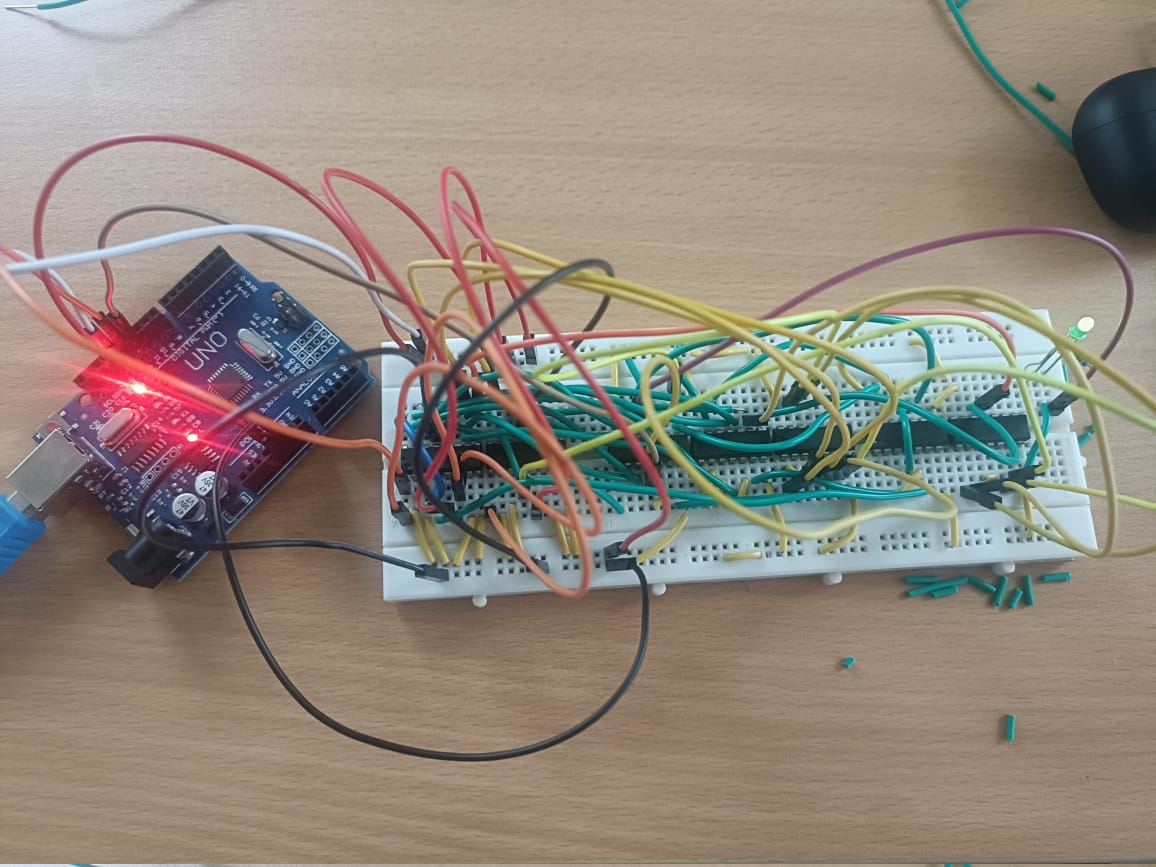
\includegraphics[width=0.7\textwidth]{figs/circuit.jpeg}
\end{figure}
\begin{figure}[H]
    \centering
    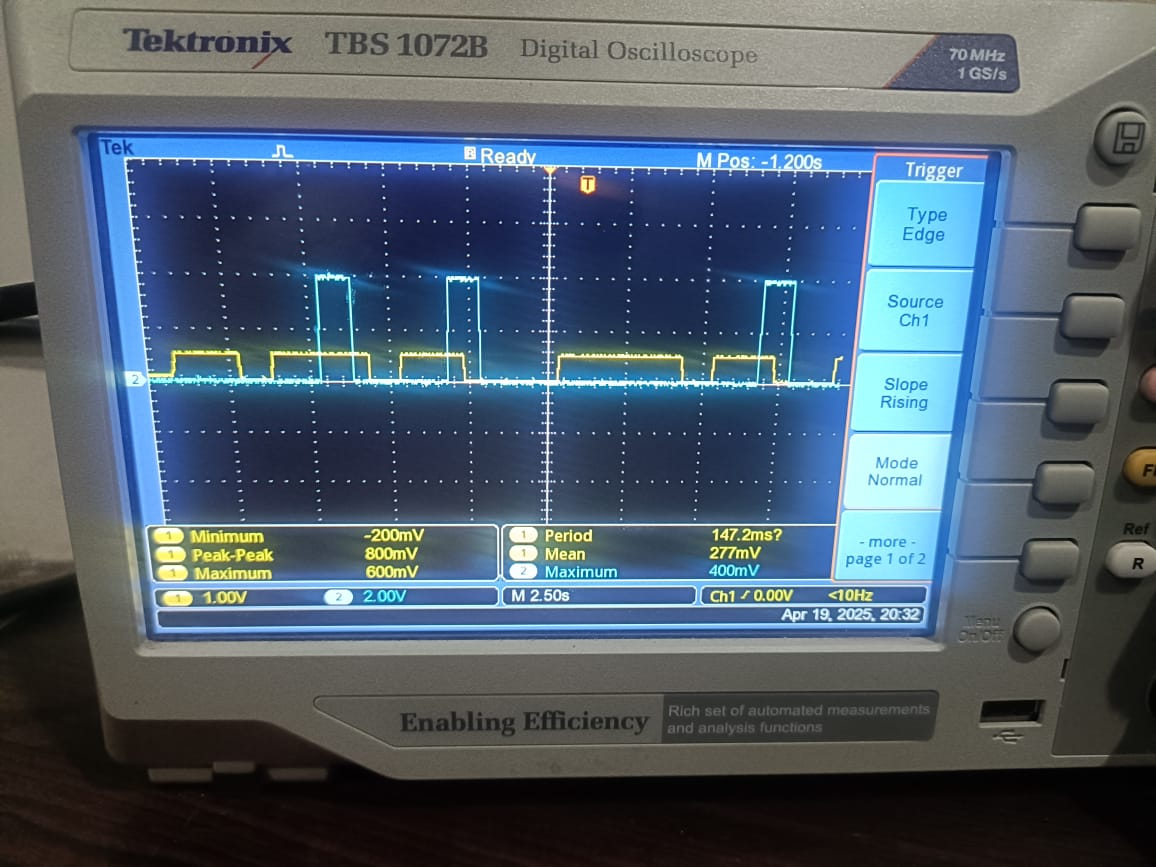
\includegraphics[width=0.7\textwidth]{figs/plot.jpeg}
\end{figure}
\section*{Result}
The FSM successfully detects the sequence \textbf{11011} and produces an output '1' whenever the sequence is detected, including overlapping instances.\\
To refer arduino code and working video refer to \\
    \url{https://github.com/ArnavYadnopavit/ElectricalLabEE1200/tree/main/LabReport9}\\
    
 \centering
 Thank you
\end{document}

